% Round-2 integration shell. No article body, no title page, no per-figure clearpage.
% Admitted: mechanisms (PR16 c959d22, not bed819cd), tables (PR18 b12cd371),
% E2 main 12-cell (PR15 05f921f2), E3--E5 (PR17 22b432ca).
% No standalone LIMIT mechanism figure and no E4 validation table.
% Do not load paper/tex/main.tex: it sets \subfigcapskip=-7pt.
% Column figures are measured boxes, not a float queue: the caption stays in
% the same box as the graphic, and the box moves to the next column when it
% does not fit. Full-width figures open a page via \twocolumn's banner.
\pdfminorversion=7
\documentclass[sigconf,nonacm]{acmart}
\usepackage{pvldb}
\settopmatter{printacmref=false,printfolios=true}
\usepackage{booktabs}
\usepackage{multirow}
\usepackage{array}
\usepackage{makecell}
\usepackage{graphicx}
\usepackage{subfigure}
\usepackage{needspace}
\usepackage{placeins}
\usepackage[ruled,vlined,linesnumbered]{algorithm2e}
\graphicspath{{../e2/out/}}
\DeclareRobustCommand{\examplelabel}{Synthetic fixture for tie-break coverage}
\SetKwProg{Fn}{procedure}{:}{}
\SetAlgoNlRelativeSize{-1}
\newcommand{\qpm}[2]{%
  {\renewcommand{\arraystretch}{0.82}%
   \begin{tabular}[c]{@{}c@{}}#1\\[-1pt]{\scriptsize$\pm$#2}\end{tabular}}}
% Single-column table inputs are minipages so Table 1 and Table 2 can sit
% side by side inside one table*. Their captions stay inside that float.
\makeatletter
\renewenvironment{table}[1][]{%
  \noindent\begin{minipage}[t]{\linewidth}%
  \captionsetup{type=table}%
  \centering
}{%
  \end{minipage}%
}
\newsavebox{\colbox}
\newcommand{\placecol}{%
  \par
  \setbox\colbox=\hbox{\raise\dp\colbox\box\colbox}%
  % 32pt keeps the caption above the folio. A 4pt pad let one
  % column figure sit 24pt past the text block under the E2 banner.
  % A single column break stays on this page. A figure taller than the
  % column under a banner has to start the next page, or it overflows by
  % the difference (E4a is 418pt under the 394pt E2 column).
  \ifdim\ht\colbox>\@colht
    \clearpage
  \else
    \Needspace{\dimexpr\ht\colbox+\dp\colbox+8pt\relax}%
  \fi
  \noindent\usebox{\colbox}\par\smallskip
}
% Used for every single-column figure. Ignores [t] so nothing enters the
% float queue (that queue dropped E3, COVID n=100, and E4c).
\newcommand{\installcolfigure}{%
  \renewenvironment{figure}[1][]{%
    \par\setbox\colbox=\vbox\bgroup
      \hsize=\columnwidth
      \linewidth=\columnwidth
      \captionsetup{type=figure}%
      \centering
  }{%
    \egroup
    \placecol
  }%
}
\makeatother
\begin{document}
\pagestyle{plain}
% Framework is full width and flat. The banner keeps it, and its caption,
% on page 1. A figure* would be deferred.
\twocolumn[{%
  \noindent\begin{minipage}{\textwidth}
    \centering
    \captionsetup{type=figure}%
    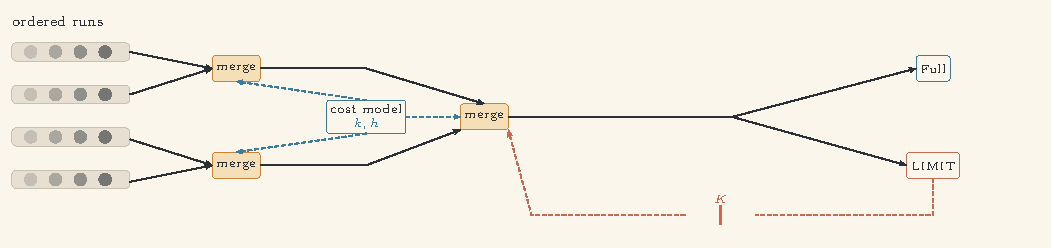
\includegraphics[width=\textwidth]{../mechanisms/framework.pdf}\par
    \captionof{figure}{Framework, full text width.}
  \end{minipage}\par
  \vskip 0.4em
}]
\typeout{TEXTHEIGHT=\the\textheight}
\typeout{COLUMNWIDTH=\the\columnwidth}
\typeout{TEXTWIDTH=\the\textwidth}
\begin{figure}[t]
  \centering
  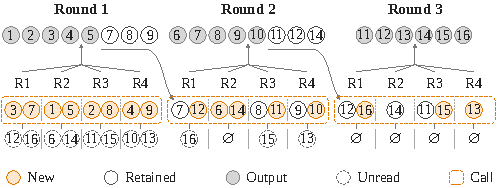
\includegraphics[width=\columnwidth]{../mechanisms/sw.pdf}
  \caption{SW, one column.}
\end{figure}
\begin{figure}[t]
  \centering
  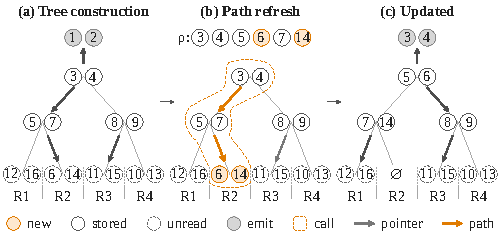
\includegraphics[width=\columnwidth]{../mechanisms/lt.pdf}
  \caption{LT(h), one column.}
\end{figure}
\begin{figure}[t]
  \centering
  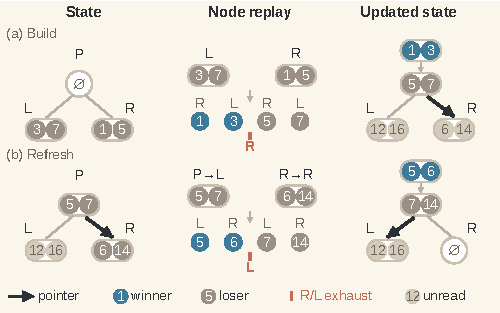
\includegraphics[width=\columnwidth]{../mechanisms/pointer.pdf}
  \caption{Pointer, one column.}
\end{figure}
\begin{table*}[t]
  \begin{minipage}[t]{0.48\textwidth}
    % Generated by recovery/tables/emit.py. Do not edit numbers by hand.
% Synthetic layout numbers, not experimental results.
\begin{table}[t]
\centering
\caption{Evaluation datasets (contract names). Corpus sizes $|D|$ and collection details are pending measurement.}
\label{tab:datasets}
\small
\setlength{\tabcolsep}{4pt}
\begin{tabular}{@{}c l c l c@{}}
\toprule
Benchmark & Dataset & $|D|$ & Domain & Queries \\
\midrule
Q9 & Q9 & --- & Review ratings & 1 \\
\midrule
\multirow{2}{*}{TREC} & DL20 & --- & Web passage retrieval & 30 \\
 & DL22 & --- & Web passage retrieval & 30 \\
\midrule
\multirow{3}{*}{BEIR} & TREC-COVID & --- & Biomedical literature & 30 \\
 & DBpedia-Entity & --- & --- & 30 \\
 & Robust04 & --- & --- & 30 \\
\bottomrule
\end{tabular}
\end{table}

  \end{minipage}\hfill
  \begin{minipage}[t]{0.48\textwidth}
    % Table 2. Call-count expressions are transcribed, not derived or checked.
\begin{table}[t]
\centering
\caption{One algorithm per row.
Horizontal rules separate sources, in order: the first four from OrderByLLM, two from ListK, LOTUS Quick, Setwise Heap, and ours.
ListK Sort/Select is one row: the Full column is LMPQSort and the LIMIT column is LMPQSelect.
Tournament is listwise tournament top~$K$.
LT($h$) is one family; $h{=}1$ is the classical tree, not another row.
Every call-count expression is an unchecked draft transcribed from the integration note.
Setwise Heap has no expression.
None of these expressions was re-derived or checked against the implementation.}
\label{tab:ranking-algorithms}
\footnotesize
\setlength{\tabcolsep}{2.2pt}
\renewcommand{\arraystretch}{1.08}
\begin{tabular*}{\columnwidth}{@{\extracolsep{\fill}}lccc@{}}
\toprule
\textbf{Algorithm} & \textbf{Type} & \textbf{Full} & \textbf{LIMIT $K$} \\
\midrule
Pointwise & Point & $\mathcal{O}(n)$ & $\mathcal{O}(n)$ \\
Ext.\ Pointwise & Point & $\mathcal{O}(n/m)$ & $\mathcal{O}(n/m)$ \\
Ext.\ Bubble & List & $\mathcal{O}(n^{2}/m^{2})$ & $\mathcal{O}(Kn/m^{2})$ \\
Ext.\ Merge & List & $\mathcal{O}((n/m)[1{+}\ell_m])$ & $\mathcal{O}((n/m)[2{+}\log(K/m)])$ \\
\midrule
ListK Sort/Select & List & $\mathcal{O}(n\log n/\chi_p{+}n)$ & $\mathcal{O}((p{+}1)n/\psi_p(\kappa))$ \\
Tournament & List & $\mathcal{O}(b_m{+}(n{-}1)\ell_m)$ & $\mathcal{O}(b_m{+}(K{-}1)\ell_m)$ \\
\midrule
Lotus Quick & Pair & $\mathcal{O}(n\log n)$ & $\mathcal{O}(n{+}K\log K)$ \\
\midrule
Setwise Heap & Set & --- & --- \\
\midrule
SW & List & $\mathcal{O}(r{+}nP(k)/\mu_{\mathrm{sw}})$ & $\mathcal{O}(r{+}KP(k)/\mu_{\mathrm{sw}})$ \\
LT($h$) & List & $\mathcal{O}(r{+}nP(k)/h)$ & $\mathcal{O}(r{+}KP(k)/h)$ \\
\bottomrule
\end{tabular*}
\vspace{0.35em}

{\footnotesize
Symbols are copied with the draft, not re-derived:
$n$ rows, $m$ list size, $K$ limit, $r{=}\lceil n/m\rceil$,
$\ell_m{=}\log(n/m)$, $b_m{=}(n{-}1)/(m{-}1)$,
$\kappa{=}K/n$, $\chi_p{=}(m{-}p)\log(p{+}1)$,
$\psi_p(\kappa){=}(m{-}p)[p{-}1{+}\kappa^{p+1}{+}(1{-}\kappa)^{p+1}]$,
and $p$ the pivot count.
$P(k)$ and $\mu_{\mathrm{sw}}$ remain the draft's own symbols.\par}
\end{table}

  \end{minipage}
\end{table*}
% Generated by src/emit.py. Do not edit numbers by hand.
% Synthetic layout, not experimental results.
\begin{table*}[t]
\centering
\caption{\examplelabel.
Synthetic layout, not a measurement.
Each cell is a mean; $\pm$ is a synthetic permutation std, not significance.
$Q$, $T$, $L$ are competition places. The ranking protocol is in \texttt{STATS.md}.}
\label{tab:exp1-full}
\begingroup
\footnotesize
\setlength{\tabcolsep}{1.6pt}
\renewcommand{\arraystretch}{0.96}
\begin{tabular*}{\textwidth}{@{\extracolsep{\fill}}l*{26}{c}@{}}
\toprule
& \multicolumn{13}{c}{\textbf{Qwen3.5-9B}} & \multicolumn{13}{c}{\textbf{Qwen3.5-27B}} \\
\cmidrule(lr){2-14}\cmidrule(lr){15-27}
Method & \multicolumn{6}{c}{Quality $\rho$} & \multicolumn{3}{c}{Tokens $\times 10^{3}$} & Lat. & \multicolumn{3}{c}{Place} & \multicolumn{6}{c}{Quality $\rho$} & \multicolumn{3}{c}{Tokens $\times 10^{3}$} & Lat. & \multicolumn{3}{c}{Place} \\
\cmidrule(lr){2-7}\cmidrule(lr){8-10}\cmidrule(lr){12-14}\cmidrule(lr){15-20}\cmidrule(lr){21-23}\cmidrule(lr){25-27}
& Q9 & DL20 & DL22 & COVID & DBP & R04 & Q9 & TREC & BEIR & s & $Q$ & $T$ & $L$ & Q9 & DL20 & DL22 & COVID & DBP & R04 & Q9 & TREC & BEIR & s & $Q$ & $T$ & $L$ \\
\midrule
Pointwise & \qpm{0.820}{0.012} & \qpm{0.820}{0.012} & \qpm{0.820}{0.012} & \qpm{0.840}{0.012} & \qpm{0.840}{0.012} & \qpm{0.840}{0.012} & 1.00 & 2.03 & 3.12 & 1.75 & 1 & 1 & 1 & \qpm{0.840}{0.012} & \qpm{0.840}{0.012} & \qpm{0.840}{0.012} & \qpm{0.860}{0.012} & \qpm{0.860}{0.012} & \qpm{0.860}{0.012} & 5.00 & 10.03 & 15.12 & 2.25 & 1 & 1 & 1 \\
Ext.\ Pointwise & \qpm{0.840}{0.013} & \qpm{0.840}{0.013} & \qpm{0.840}{0.013} & \qpm{0.820}{0.013} & \qpm{0.820}{0.013} & \qpm{0.800}{0.013} & 1.10 & 2.23 & 3.42 & 2.15 & 2 & 2 & 2 & \qpm{0.860}{0.013} & \qpm{0.860}{0.013} & \qpm{0.860}{0.013} & \qpm{0.840}{0.013} & \qpm{0.840}{0.013} & \qpm{0.820}{0.013} & 5.10 & 10.23 & 15.42 & 2.65 & 2 & 2 & 2 \\
Ext.\ Bubble & \qpm{0.800}{0.014} & \qpm{0.800}{0.014} & \qpm{0.800}{0.014} & \qpm{0.800}{0.014} & \qpm{0.780}{0.014} & \qpm{0.820}{0.014} & 1.20 & 2.43 & 3.72 & 2.55 & 3 & 3 & 3 & \qpm{0.820}{0.014} & \qpm{0.820}{0.014} & \qpm{0.820}{0.014} & \qpm{0.820}{0.014} & \qpm{0.800}{0.014} & \qpm{0.840}{0.014} & 5.20 & 10.43 & 15.72 & 3.05 & 3 & 3 & 3 \\
Ext.\ Merge & \qpm{0.780}{0.015} & \qpm{0.780}{0.015} & \qpm{0.780}{0.015} & \qpm{0.780}{0.015} & \qpm{0.800}{0.015} & \qpm{0.780}{0.015} & 1.30 & 2.63 & 4.02 & 2.95 & 4 & 4 & 4 & \qpm{0.800}{0.015} & \qpm{0.800}{0.015} & \qpm{0.800}{0.015} & \qpm{0.800}{0.015} & \qpm{0.820}{0.015} & \qpm{0.800}{0.015} & 5.30 & 10.63 & 16.02 & 3.45 & 4 & 4 & 4 \\
\midrule
ListK Sort & \qpm{0.760}{0.016} & \qpm{0.760}{0.016} & \qpm{0.760}{0.016} & \qpm{0.760}{0.016} & \qpm{0.760}{0.016} & \qpm{0.760}{0.016} & 1.40 & 3.10 & 6.00 & 3.35 & 5 & 6 & 5 & \qpm{0.780}{0.016} & \qpm{0.780}{0.016} & \qpm{0.780}{0.016} & \qpm{0.780}{0.016} & \qpm{0.780}{0.016} & \qpm{0.780}{0.016} & 5.40 & 11.10 & 18.00 & 3.85 & 5 & 6 & 5 \\
Tournament & \qpm{0.740}{0.017} & \qpm{0.740}{0.017} & \qpm{0.740}{0.017} & \qpm{0.740}{0.017} & \qpm{0.740}{0.017} & \qpm{0.740}{0.017} & 1.41 & 3.12 & 5.10 & 3.75 & 6 & 5 & 6 & \qpm{0.760}{0.017} & \qpm{0.760}{0.017} & \qpm{0.760}{0.017} & \qpm{0.760}{0.017} & \qpm{0.760}{0.017} & \qpm{0.760}{0.017} & 5.41 & 11.12 & 17.10 & 4.25 & 6 & 5 & 6 \\
\midrule
Lotus Quick & \qpm{0.720}{0.018} & \qpm{0.720}{0.018} & \qpm{0.720}{0.018} & \qpm{0.720}{0.018} & \qpm{0.720}{0.018} & \qpm{0.720}{0.018} & 3.00 & 6.03 & 9.12 & 4.15 & 7 & 7 & 7 & \qpm{0.740}{0.018} & \qpm{0.740}{0.018} & \qpm{0.740}{0.018} & \qpm{0.740}{0.018} & \qpm{0.740}{0.018} & \qpm{0.740}{0.018} & 7.00 & 14.03 & 21.12 & 4.65 & 7 & 7 & 7 \\
\midrule
Setwise Heap & \qpm{0.700}{0.019} & \qpm{0.700}{0.019} & \qpm{0.700}{0.019} & \qpm{0.700}{0.019} & \qpm{0.700}{0.019} & \qpm{0.700}{0.019} & 3.10 & 6.23 & 9.42 & 4.55 & 8 & 8 & 8 & \qpm{0.720}{0.019} & \qpm{0.720}{0.019} & \qpm{0.720}{0.019} & \qpm{0.720}{0.019} & \qpm{0.720}{0.019} & \qpm{0.720}{0.019} & 7.10 & 14.23 & 21.42 & 5.05 & 8 & 8 & 8 \\
\midrule
SW & \qpm{0.680}{0.020} & \qpm{0.670}{0.030} & \qpm{0.680}{0.020} & \qpm{0.680}{0.020} & \qpm{0.680}{0.020} & \qpm{0.680}{0.020} & 3.20 & 6.43 & 9.72 & 4.95 & 9 & 9 & 9 & \qpm{0.700}{0.020} & \qpm{0.690}{0.030} & \qpm{0.700}{0.020} & \qpm{0.700}{0.020} & \qpm{0.700}{0.020} & \qpm{0.700}{0.020} & 7.20 & 14.43 & 21.72 & 5.45 & 9 & 9 & 9 \\
LT($h$) & \qpm{0.660}{0.021} & \qpm{0.670}{0.011} & \qpm{0.660}{0.021} & \qpm{0.660}{0.021} & \qpm{0.660}{0.021} & \qpm{0.660}{0.021} & 3.30 & 6.63 & 10.02 & 5.35 & 10 & 10 & 10 & \qpm{0.680}{0.021} & \qpm{0.690}{0.011} & \qpm{0.680}{0.021} & \qpm{0.680}{0.021} & \qpm{0.680}{0.021} & \qpm{0.680}{0.021} & 7.30 & 14.63 & 22.02 & 5.85 & 10 & 10 & 10 \\
\bottomrule
\end{tabular*}
\endgroup
\end{table*}

% Flush only the tables that already fill a page. LIMIT is not a float:
% it is the banner of the next page, and the algorithms continue under it.
\FloatBarrier
\twocolumn[{%
  \begingroup
  \renewenvironment{table*}[1][]{%
    \noindent\begin{minipage}{\textwidth}%
    \captionsetup{type=table}%
    \centering
  }{\end{minipage}\par}%
  % Generated by src/emit.py. Do not edit numbers by hand.
% Synthetic layout, not experimental results.
\begin{table*}[t]
\centering
\caption{LIMIT $K{=}10$ (nDCG@10). Synthetic layout fixture, not measurements.
Quality is mean $\pm$ permutation std, not significance.
Tokens denote logical end-to-end Total (input + output), not the framework's merge-input-only objective;
columns sum dataset means: Q9; TREC = DL20 + DL22; BEIR = COVID + DBP + R04.
Latency is the equal-weight mean over six datasets, in seconds.
$Q,T,L$ are six-dataset competition places (\texttt{STATS.md}).
Bold/underline mark first/second competition place within each displayed column; ties share emphasis.
Model labels are requested labels; deployment manifests remain unverified. The ListK row is ListK Select.}
\label{tab:exp1-limit}
\begingroup
\fontsize{6.4}{8.2}\fontfamily{qhv}\fontseries{c}\selectfont
\renewcommand{\qpm}[2]{\mbox{\IfBeginWith{#1}{0.}{\StrGobbleLeft{#1}{1}}{#1}{\fontsize{5.8}{6.5}\selectfont\textpm\IfBeginWith{#2}{0.}{\StrGobbleLeft{#2}{1}}{#2}}}}
\setlength{\tabcolsep}{0.4pt}
\renewcommand{\arraystretch}{1.18}
\begin{tabular*}{\textwidth}{@{\extracolsep{\fill}}l!{\hspace{1.5pt}}c*{5}{!{\hspace{2.4pt}}c}!{\hspace{2pt}}c*{4}{!{\hspace{1.2pt}}c}*{2}{@{\hspace{1.75pt}}c}!{\hspace{3pt}}c*{5}{!{\hspace{2.4pt}}c}!{\hspace{2pt}}c*{4}{!{\hspace{1.2pt}}c}*{2}{@{\hspace{1.75pt}}c}@{}}
\toprule
& \multicolumn{13}{c}{\fontsize{7}{8}\selectfont\textbf{Qwen3.5-9B}} & \multicolumn{13}{c}{\fontsize{7}{8}\selectfont\textbf{Qwen3.8-27B}} \\
\cmidrule(lr){2-14}\cmidrule(lr){15-27}
Method & \multicolumn{6}{c}{nDCG@10} & \multicolumn{3}{c}{Tokens $\times 10^{3}$} & Lat. & \multicolumn{3}{c}{Place} & \multicolumn{6}{c}{nDCG@10} & \multicolumn{3}{c}{Tokens $\times 10^{3}$} & Lat. & \multicolumn{3}{c}{Place} \\
\cmidrule(lr){2-7}\cmidrule(lr){8-10}\cmidrule(lr){12-14}\cmidrule(lr){15-20}\cmidrule(lr){21-23}\cmidrule(lr){25-27}
& Q9 & DL20 & DL22 & COVID & DBP & R04 & Q9 & TREC & BEIR & s & $Q$ & $T$ & $L$ & Q9 & DL20 & DL22 & COVID & DBP & R04 & Q9 & TREC & BEIR & s & $Q$ & $T$ & $L$ \\
\midrule
Pointwise & \underline{\qpm{0.780}{0.012}} & \underline{\qpm{0.780}{0.012}} & \underline{\qpm{0.780}{0.012}} & \textbf{\qpm{0.800}{0.012}} & \textbf{\qpm{0.800}{0.012}} & \textbf{\qpm{0.800}{0.012}} & \textbf{1.70} & \textbf{3.43} & \textbf{5.22} & \textbf{2.05} & \textbf{1} & \textbf{1} & \textbf{1} & \underline{\qpm{0.800}{0.012}} & \underline{\qpm{0.800}{0.012}} & \underline{\qpm{0.800}{0.012}} & \textbf{\qpm{0.820}{0.012}} & \textbf{\qpm{0.820}{0.012}} & \textbf{\qpm{0.820}{0.012}} & \textbf{5.70} & \textbf{11.43} & \textbf{17.22} & \textbf{2.55} & \textbf{1} & \textbf{1} & \textbf{1} \\
Ext. Pointwise & \textbf{\qpm{0.800}{0.013}} & \textbf{\qpm{0.800}{0.013}} & \textbf{\qpm{0.800}{0.013}} & \underline{\qpm{0.780}{0.013}} & \underline{\qpm{0.780}{0.013}} & \qpm{0.760}{0.013} & \underline{1.80} & \underline{3.63} & \underline{5.52} & \underline{2.45} & \underline{2} & \underline{2} & \underline{2} & \textbf{\qpm{0.820}{0.013}} & \textbf{\qpm{0.820}{0.013}} & \textbf{\qpm{0.820}{0.013}} & \underline{\qpm{0.800}{0.013}} & \underline{\qpm{0.800}{0.013}} & \qpm{0.780}{0.013} & \underline{5.80} & \underline{11.63} & \underline{17.52} & \underline{2.95} & \underline{2} & \underline{2} & \underline{2} \\
Ext. Bubble & \qpm{0.760}{0.014} & \qpm{0.760}{0.014} & \qpm{0.760}{0.014} & \qpm{0.760}{0.014} & \qpm{0.740}{0.014} & \underline{\qpm{0.780}{0.014}} & 1.90 & 3.83 & 5.82 & 2.85 & 3 & 3 & 3 & \qpm{0.780}{0.014} & \qpm{0.780}{0.014} & \qpm{0.780}{0.014} & \qpm{0.780}{0.014} & \qpm{0.760}{0.014} & \underline{\qpm{0.800}{0.014}} & 5.90 & 11.83 & 17.82 & 3.35 & 3 & 3 & 3 \\
Ext. Merge & \qpm{0.740}{0.015} & \qpm{0.740}{0.015} & \qpm{0.740}{0.015} & \qpm{0.740}{0.015} & \qpm{0.760}{0.015} & \qpm{0.740}{0.015} & 2.00 & 4.03 & 6.12 & 3.25 & 4 & 4 & 4 & \qpm{0.760}{0.015} & \qpm{0.760}{0.015} & \qpm{0.760}{0.015} & \qpm{0.760}{0.015} & \qpm{0.780}{0.015} & \qpm{0.760}{0.015} & 6.00 & 12.03 & 18.12 & 3.75 & 4 & 4 & 4 \\
\midrule
ListK Select & \qpm{0.720}{0.016} & \qpm{0.720}{0.016} & \qpm{0.720}{0.016} & \qpm{0.720}{0.016} & \qpm{0.720}{0.016} & \qpm{0.720}{0.016} & 2.10 & 4.50 & 8.10 & 3.65 & 5 & 6 & 5 & \qpm{0.740}{0.016} & \qpm{0.740}{0.016} & \qpm{0.740}{0.016} & \qpm{0.740}{0.016} & \qpm{0.740}{0.016} & \qpm{0.740}{0.016} & 6.10 & 12.50 & 20.10 & 4.15 & 5 & 6 & 5 \\
Tournament & \qpm{0.700}{0.017} & \qpm{0.700}{0.017} & \qpm{0.700}{0.017} & \qpm{0.700}{0.017} & \qpm{0.700}{0.017} & \qpm{0.700}{0.017} & 2.11 & 4.52 & 7.20 & 4.05 & 6 & 5 & 6 & \qpm{0.720}{0.017} & \qpm{0.720}{0.017} & \qpm{0.720}{0.017} & \qpm{0.720}{0.017} & \qpm{0.720}{0.017} & \qpm{0.720}{0.017} & 6.11 & 12.52 & 19.20 & 4.55 & 6 & 5 & 6 \\
\midrule
Lotus Quick & \qpm{0.680}{0.018} & \qpm{0.680}{0.018} & \qpm{0.680}{0.018} & \qpm{0.680}{0.018} & \qpm{0.680}{0.018} & \qpm{0.680}{0.018} & 3.70 & 7.43 & 11.22 & 4.45 & 7 & 7 & 7 & \qpm{0.700}{0.018} & \qpm{0.700}{0.018} & \qpm{0.700}{0.018} & \qpm{0.700}{0.018} & \qpm{0.700}{0.018} & \qpm{0.700}{0.018} & 7.70 & 15.43 & 23.22 & 4.95 & 7 & 7 & 7 \\
\midrule
Setwise Heap & \qpm{0.660}{0.019} & \qpm{0.660}{0.019} & \qpm{0.660}{0.019} & \qpm{0.660}{0.019} & \qpm{0.660}{0.019} & \qpm{0.660}{0.019} & 3.80 & 7.63 & 11.52 & 4.85 & 8 & 8 & 8 & \qpm{0.680}{0.019} & \qpm{0.680}{0.019} & \qpm{0.680}{0.019} & \qpm{0.680}{0.019} & \qpm{0.680}{0.019} & \qpm{0.680}{0.019} & 7.80 & 15.63 & 23.52 & 5.35 & 8 & 8 & 8 \\
\midrule
SW & \qpm{0.640}{0.020} & \qpm{0.630}{0.030} & \qpm{0.640}{0.020} & \qpm{0.640}{0.020} & \qpm{0.640}{0.020} & \qpm{0.640}{0.020} & 3.90 & 7.83 & 11.82 & 5.25 & 9 & 9 & 9 & \qpm{0.660}{0.020} & \qpm{0.650}{0.030} & \qpm{0.660}{0.020} & \qpm{0.660}{0.020} & \qpm{0.660}{0.020} & \qpm{0.660}{0.020} & 7.90 & 15.83 & 23.82 & 5.75 & 9 & 9 & 9 \\
LT($h$) & \qpm{0.620}{0.021} & \qpm{0.630}{0.011} & \qpm{0.620}{0.021} & \qpm{0.620}{0.021} & \qpm{0.620}{0.021} & \qpm{0.620}{0.021} & 4.00 & 8.03 & 12.12 & 5.65 & 10 & 10 & 10 & \qpm{0.640}{0.021} & \qpm{0.650}{0.011} & \qpm{0.640}{0.021} & \qpm{0.640}{0.021} & \qpm{0.640}{0.021} & \qpm{0.640}{0.021} & 8.00 & 16.03 & 24.12 & 6.15 & 10 & 10 & 10 \\
\bottomrule
\end{tabular*}
\endgroup
\end{table*}
%
  \endgroup
}]
% Place algorithm 4 at the top of the other column. Otherwise 3, 4, and 5
% stack in the left column and the right column stays empty.
\makeatletter
\newcount\algplaced
\let\savednewcommand\newcommand
\let\newcommand\providecommand
\providecommand{\algcolstart}{%
  \par
  \begin{lrbox}{\algcolbox}%
  \begin{minipage}[t]{\columnwidth}%
  \@twocolumnfalse
}
\providecommand{\algcolend}{%
  \end{minipage}%
  \end{lrbox}%
  \setbox\algcolbox=\hbox{\raise\dp\algcolbox\box\algcolbox}%
  \ifnum\algplaced=3
    \newpage
  \fi
  \Needspace{\dimexpr\ht\algcolbox+\dp\algcolbox+6pt\relax}%
  \noindent\usebox{\algcolbox}\par\smallskip
  \global\advance\algplaced by 1
}
\makeatother
% Default path: evidence off, no input shuffle.
% The objective is estimated merge input tokens; no unverified cost formula is used.
% Full materializes each pass. LIMIT pulls the same groups and stops at K.
% h=1 is LT(h), not a second family.
\DontPrintSemicolon
\newcommand{\Rank}{\mbox{\textsc{ListwiseRank}}}
\newcommand{\Replay}{\mbox{\textsc{Replay}}}
\newcommand{\Refresh}{\mbox{\textsc{Refresh}}}
\newcommand{\MergeGroup}{\mbox{\textsc{MergeGroup}}}
\newcommand{\Expect}{\ensuremath{\mathrm{Expect}}}
\SetKwProg{Fn}{procedure}{:}{}
\SetAlgoNlRelativeSize{-1}
\SetAlFnt{\footnotesize}
\SetAlCapFnt{\footnotesize}
\SetAlgoSkip{}
\SetAlgoInsideSkip{}
\makeatletter
% algorithm2e rejects [H] in two-column mode. Measure the column box, then
% move the whole algorithm to the next column when it does not fit.
% \Needspace comes from the integration preamble; the fallback keeps the
% specialist preview compiling if that package was not loaded.
\providecommand{\Needspace}[1]{}
\newsavebox{\algcolbox}
\newcommand{\algcolstart}{%
  \par
  \begin{lrbox}{\algcolbox}%
  \begin{minipage}[t]{\columnwidth}%
  \@twocolumnfalse
}
\newcommand{\algcolend}{%
  \end{minipage}%
  \end{lrbox}%
  % minipage[t] stores the body as depth. Raise it so the page builder
  % sees the whole algorithm above the baseline and cannot hang off the page.
  \setbox\algcolbox=\hbox{\raise\dp\algcolbox\box\algcolbox}%
  \typeout{ALGBOX ht=\the\ht\algcolbox dp=\the\dp\algcolbox}%
  \Needspace{\dimexpr\ht\algcolbox+\dp\algcolbox+6pt\relax}%
  \noindent\usebox{\algcolbox}\par\smallskip
}
\makeatother

% Paper abstraction: default no-evidence/no-shuffle path; no execution change.
{\footnotesize\raggedright
\noindent\textit{Conventions.}
$\Rank_\phi(X)$ orders real rows best first; $|X|\le1$ needs no call.
$\operatorname{take}_q$ reads at most $q$ rows ($q=\infty$: drain).
$\Vert$ concatenates in order; $B_u$ is run $u$'s subsequence in $B$.
$\operatorname{unread}(u)$ means unread supply remains.
$\mathcal L(X)$ ranks $X$ once to order the active heads ($\rho$).
$[\bot_a]^r$ means $r$ virtual entries tagged $a$; $\operatorname{real}$ removes them.
$\MergeGroup$ forwards singletons; Full materializes each pass, LIMIT pulls and truncates only the root.
$\mathcal F$ is the feasible set; estimates use run lengths, token profile, mode and $K$.
\textsc{HalvingTree} rounds the left size up; \textsc{Cut} takes maximal subtrees within the frontier bound.\par}

\algcolstart
\begin{algorithm}[H]
\caption{External Merge Group via $k$-Way Merge}
\label{alg:semantic_external_merge}
\KwIn{rows $D$, instruction $\phi$, capacity $m$, mode Full or LIMIT, bound $K$ (default $\infty$)}
\lIf{$D=\varnothing$ or $K=0$}{\Return $[\,]$}
$\mathcal R\leftarrow[\Rank_\phi(C):C\in\operatorname{Chunks}_m(D)]$\;
\lIf{$|\mathcal R|=1$}{\Return $\operatorname{take}_K(\mathcal R_1)$}
$(f,k,h)\leftarrow\arg\min_{(f,k,h)\in\mathcal F}\widehat C_{\rm merge}(f,k,h)$\;
\While{$|\mathcal R|>1$}{
  $\mathcal G\leftarrow\operatorname{Chunks}_k(\mathcal R)$\;
  $\mathcal R'\leftarrow[\MergeGroup_{f,h}(G):G\in\mathcal G]$\;
  \lIf{Full}{$\mathcal R'\leftarrow[\operatorname{materialize}(S):S\in\mathcal R']$}
  $\mathcal R\leftarrow\mathcal R'$\;
}
\Return $\operatorname{take}_K(\mathcal R_1)$\;
\end{algorithm}
\algcolend

\algcolstart
\begin{algorithm}[H]
\caption{Sliding-Window Semantic $k$-Way Merge}
\label{alg:sliding_window_kway_group_merge}
\KwIn{$2\le g\le m$ runs; adaptive quota or fixed $1\le h\le\lfloor m/g\rfloor$}
$B\leftarrow[\,]$\;
\While{$B\ne[\,]$ or some run is unread}{
  $A\leftarrow\{u:|B_u|>0\ \lor\ \operatorname{unread}(u)\}$\;
  $q\leftarrow h$ if fixed, else $\lfloor m/|A|\rfloor$\;
  \ForEach{$u\in A$ in run order}{
    $B\leftarrow B\Vert\operatorname{take}_{\max(0,q-|B_u|)}(R_u)$\;
  }
  \lIf{adaptive}{round-robin refill $B$ up to $|A|q$ rows}
  \lIf{$B=[\,]$}{stop}
  $A\leftarrow\{u:|B_u|>0\ \lor\ \operatorname{unread}(u)\}$\;
  \lIf{$A=\{u\}$}{yield $B_u\Vert\operatorname{take}_\infty(R_u)$; stop}
  $O\leftarrow\Rank_\phi(B)$\;
  $J\leftarrow\{j:\exists u,\ \operatorname{unread}(u),\ |B_u|>0,$\;
  \Indp $\qquad |(O_{1:j})_u|=|B_u|\}$\;\Indm
  $t\leftarrow\min(J\cup\{|O|\})$\;
  yield $O_{1:t}$; $B\leftarrow\operatorname{stableRemove}(B,O_{1:t})$\;
}
\end{algorithm}
\algcolend

\algcolstart
\begin{algorithm}[H]
\caption{Loser-Tree Semantic $k$-Way Merge}
\label{alg:loser_tree_kway_group_merge}
\KwIn{$g\ge2$ runs, $h\ge1$, $(1+\lceil\log_2 g\rceil)h\le m$}
$T\leftarrow\operatorname{HalvingTree}(R_1,\ldots,R_g)$; $F\leftarrow\operatorname{leaves}(T)$\;
\ForEach{$u\in F$}{$S_u\leftarrow\operatorname{take}_h(R_u)$}
\While{$F\ne\{\mathrm{root}\}$}{
  $\mathcal B\leftarrow\operatorname{Cut}(T,F,\lfloor m/h\rfloor)$\;
  \ForEach{$b\in\mathcal B$ with more than one frontier leaf}{
    $X\leftarrow\mathop{\Vert}_{u\in F\cap b}^{\rm left\ to\ right}S_u$;
    $\rho\leftarrow\mathcal L(X)$\;
    \ForEach{new internal $v$ of $b$, bottom-up}{
      $(S_v,\ell_v,p_v)\leftarrow\Replay(v,S_{v_L},S_{v_R},\rho)$\;
    }
  }
  $F\leftarrow\{\operatorname{root}(b):b\in\mathcal B\}$\;
}
\While{$S_{\rm root}\ne[\,]$}{yield $S_{\rm root}$; $S_{\rm root}\leftarrow\Refresh(T)$}
\end{algorithm}
\algcolend

\algcolstart
\begin{algorithm}[H]
\caption{Node Replay}
\label{alg:replay_segment_node}
\KwIn{node $v$, slots $s_L,s_R$ with $|s_L|,|s_R|\le h$, rank map $\rho$}
$Z\leftarrow\operatorname{sort}_\rho(s_L\Vert s_R)$, retaining slot tags\;
$Z\leftarrow Z\Vert[\bot_L]^{h-|s_L|}\Vert[\bot_R]^{h-|s_R|}$\;
$j^*\leftarrow\min\{j:\max_{a\in\{L,R\}}|(Z_{1:j})_a|=h\}$\;
$p\leftarrow v_{\operatorname{slot}(Z_{j^*})}$\;
\Return $(\operatorname{real}(Z_{1:h}),\operatorname{real}(Z_{h+1:}),p)$\;
\end{algorithm}
\algcolend

\algcolstart
\begin{algorithm}[H]
\caption{Path Refresh}
\label{alg:refresh_loser_tree_path}
\KwIn{LT($h$) $T$ after root emission; losers $\ell_v$ and child pointers $p_v$ at internal nodes}
$P\leftarrow[\,]$; $u\leftarrow\operatorname{root}(T)$\;
\While{$u$ is internal}{$P\leftarrow P\Vert[u]$; $u\leftarrow p_u$}
$S\leftarrow\operatorname{take}_h(R_u)$\;
$X\leftarrow S\Vert\mathop{\Vert}_{v\in P}\ell_v$; $\rho\leftarrow\mathcal L(X)$\;
\ForEach{$v\in\operatorname{reverse}(P)$}{
  $(s_L,s_R)\leftarrow(S,\ell_v)$ if $p_v=v_L$, else $(\ell_v,S)$\;
  $(S,\ell_v,p_v)\leftarrow\Replay(v,s_L,s_R,\rho)$\;
}
\Return $S$\;
\end{algorithm}
\algcolend

\let\newcommand\savednewcommand
% E2 stays at the admitted panel size (0.33 of the sigconf column).
% It is a banner, not a cleared page: column figures continue under it
% when they fit. Do not add \clearpage here.
\renewenvironment{figure*}[1][]{%
  \noindent\begin{minipage}{\textwidth}%
  \setlength{\columnwidth}{241.14749pt}%
  \captionsetup{type=figure}%
  \setlength{\abovecaptionskip}{2pt}%
  \setlength{\belowcaptionskip}{0pt}%
  \centering
}{%
  \end{minipage}\par
}
\twocolumn[{%
  \graphicspath{{../e2/out/}}%
  \setlength{\columnwidth}{241.14749pt}%
  \setlength{\linewidth}{\textwidth}%
  % Structure follows unpacked-paper/exp.tex fig:exp5-m (417--472):
% 0.8\linewidth legend, \vspace{-2ex}, 0.33\columnwidth cells, \hspace{-2.5ex},
% a blank line between the two rows. Image paths and short titles differ.
% Not the missing 3D k-sweep float. Heights are synthetic.
\begin{figure*}[t]
  \centering

  
\includegraphics[width=0.8\linewidth]{e2-legend.pdf}

  \vspace{-2ex}

  \subfigure[Syn-A, LT, Full]{
      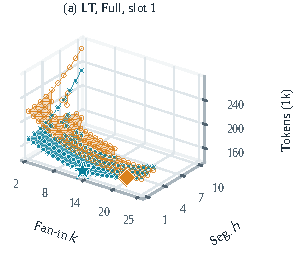
\includegraphics[width=0.33\columnwidth]{panels/p01.pdf}
  }
  \hspace{-2.5ex}
  \subfigure[Syn-B, LT, Full]{
      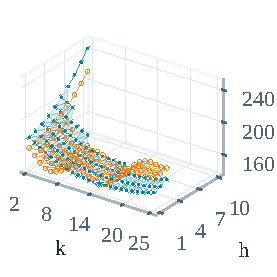
\includegraphics[width=0.33\columnwidth]{panels/p02.pdf}
  }
  \hspace{-2.5ex}
  \subfigure[Syn-C, LT, Full]{
      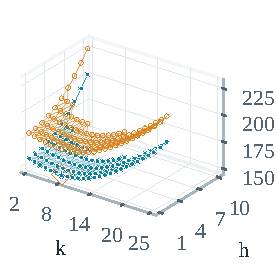
\includegraphics[width=0.33\columnwidth]{panels/p03.pdf}
  }
  \subfigure[Syn-D, LT, LIMIT10]{
      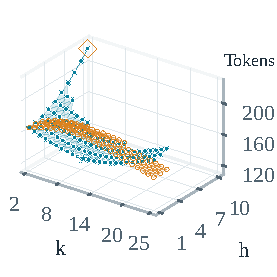
\includegraphics[width=0.33\columnwidth]{panels/p04.pdf}
  }
  \hspace{-2.5ex}
  \subfigure[Syn-E, LT, LIMIT10]{
      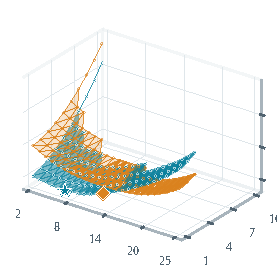
\includegraphics[width=0.33\columnwidth]{panels/p05.pdf}
  }
  \hspace{-2.5ex}
  \subfigure[Syn-F, LT, LIMIT10]{
      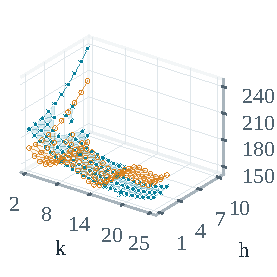
\includegraphics[width=0.33\columnwidth]{panels/p06.pdf}
  }

  \subfigure[Syn-G, SW, Full]{
      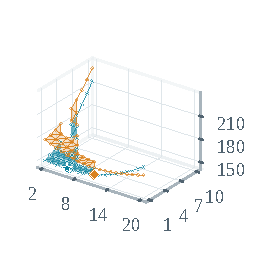
\includegraphics[width=0.33\columnwidth]{panels/p07.pdf}
  }
  \hspace{-2.5ex}
  \subfigure[Syn-H, SW, Full]{
      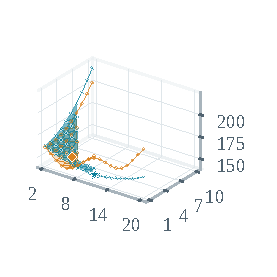
\includegraphics[width=0.33\columnwidth]{panels/p08.pdf}
  }
  \hspace{-2.5ex}
  \subfigure[Syn-I, SW, Full]{
      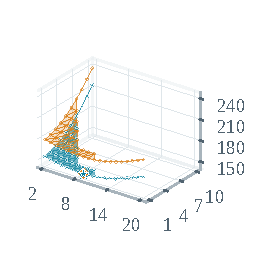
\includegraphics[width=0.33\columnwidth]{panels/p09.pdf}
  }
  \subfigure[Syn-J, SW, LIMIT10]{
      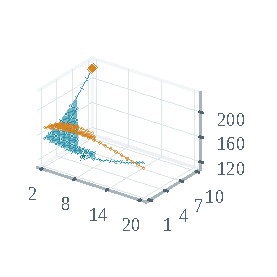
\includegraphics[width=0.33\columnwidth]{panels/p10.pdf}
  }
  \hspace{-2.5ex}
  \subfigure[Syn-K, SW, LIMIT10]{
      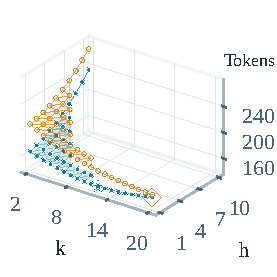
\includegraphics[width=0.33\columnwidth]{panels/p11.pdf}
  }
  \hspace{-2.5ex}
  \subfigure[Syn-L, SW, LIMIT10]{
      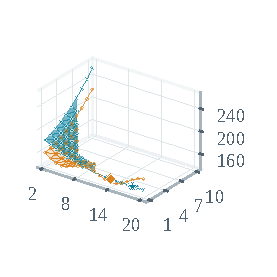
\includegraphics[width=0.33\columnwidth]{panels/p12.pdf}
  }

  \caption{Synthetic schematic cost (tokens $\times 10^{3}$), not experimental results.}
  \label{fig:e2-surface-exp5-12}
\end{figure*}
%
  % The banner's depth is about 24pt past the height LaTeX reserves.
  % This skip is empty space under the caption, not a rescale of the panels.
}]
\installcolfigure
{\graphicspath{{../experiments/figures/e3/}}%
% E3 scale scaffold. Single-column container copied from the original
% fig:exp4-topk (exp.tex, Figure 8): legend above, panels at 0.25\columnwidth.
% SW / LT / Full / LIMIT / predicted / measured are set here, not inside the PDFs.
% Not inserted into the paper. Graphic path: figures/e3/
\begin{figure}[t]
  % Local to this float. The old paper sets \subfigcapskip=-7pt, which
  % pulls n / 10k under the subcaption. Do not inherit that value.
  \setlength{\subfigcapskip}{1pt}
  \centering
  
\includegraphics[width=\columnwidth]{e3-legend.pdf}\par
  \vspace{-0.45em}
  % Two short lines: a single line does not fit in 0.25 column.
  % Fig.~8 uses \hspace{-2.6ex}. At this panel's margins that shift
  % covers the following panel's "10k" (sigconf preview), so the
  % four boxes sit edge to edge instead.
  \newcommand{\eiiicap}[2]{\protect\shortstack{\scriptsize #1\\#2}}%
  \subfigure[\eiiicap{SW, Full}{predicted}]{%
    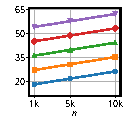
\includegraphics[width=0.25\columnwidth]{e3-sw-full-predicted.pdf}}%
  \subfigure[\eiiicap{SW, LIMIT}{predicted}]{%
    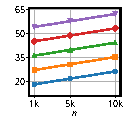
\includegraphics[width=0.25\columnwidth]{e3-sw-limit10-predicted.pdf}}%
  \subfigure[\eiiicap{LT, Full}{predicted}]{%
    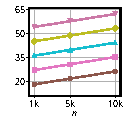
\includegraphics[width=0.25\columnwidth]{e3-lt-full-predicted.pdf}}%
  \subfigure[\eiiicap{LT, LIMIT}{predicted}]{%
    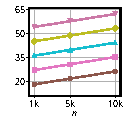
\includegraphics[width=0.25\columnwidth]{e3-lt-limit10-predicted.pdf}}%
  \\[0.15em]
  \subfigure[\eiiicap{SW, Full}{measured}]{%
    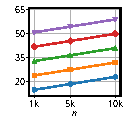
\includegraphics[width=0.25\columnwidth]{e3-sw-full-measured.pdf}}%
  \subfigure[\eiiicap{SW, LIMIT}{measured}]{%
    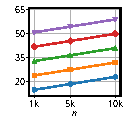
\includegraphics[width=0.25\columnwidth]{e3-sw-limit10-measured.pdf}}%
  \subfigure[\eiiicap{LT, Full}{measured}]{%
    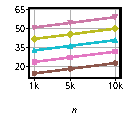
\includegraphics[width=0.25\columnwidth]{e3-lt-full-measured.pdf}}%
  \subfigure[\eiiicap{LT, LIMIT}{measured}]{%
    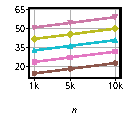
\includegraphics[width=0.25\columnwidth]{e3-lt-limit10-measured.pdf}}%
  \caption{Synthetic scale scaffold, not a measured token cost.
  Top row predicted, bottom row measured.
  Left legend entries are the SW series $(k,h)$; right entries are the LT series.
  The horizontal position is linear in $n\in\{1\mathrm{k},5\mathrm{k},10\mathrm{k}\}$;
  the vertical axis is one shared layout scale.
  Panel box is $0.25$ column.}
  \label{fig:e3-scale}
\end{figure}
}
{\graphicspath{{../experiments/figures/e4a/}}%
% E4a. One single-column figure per dataset and n.
% Not inserted into the paper. Graphic path: figures/e4a/
\newcommand{\eFourAnote}{%
  Synthetic layout sample, not an experimental result.
  A star is the predicted configuration and a diamond the measured minimum, both at that configuration's measured height.
  The minimum is over the displayed categories only, not the legal domain.
  Real display points are still deferred.%
}

\begin{figure}[t]
  \centering
  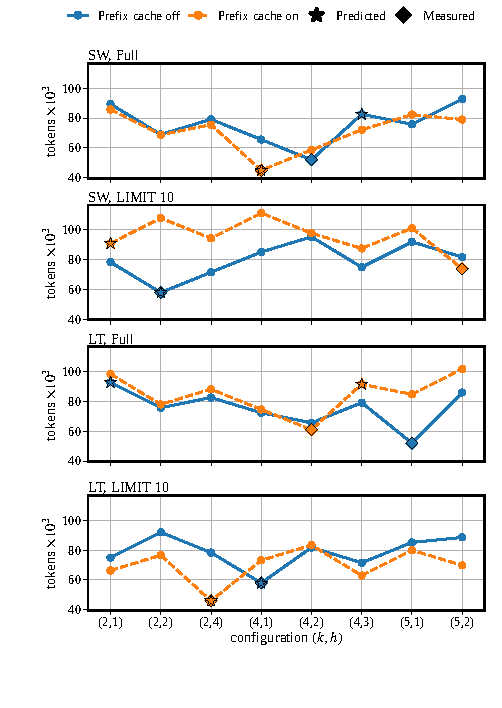
\includegraphics[width=\columnwidth]{e4a-dl20-n100.pdf}
  \caption{DL20, $n{=}100$. \eFourAnote}
  \label{fig:e4a-dl20-n100}
\end{figure}

\begin{figure}[t]
  \centering
  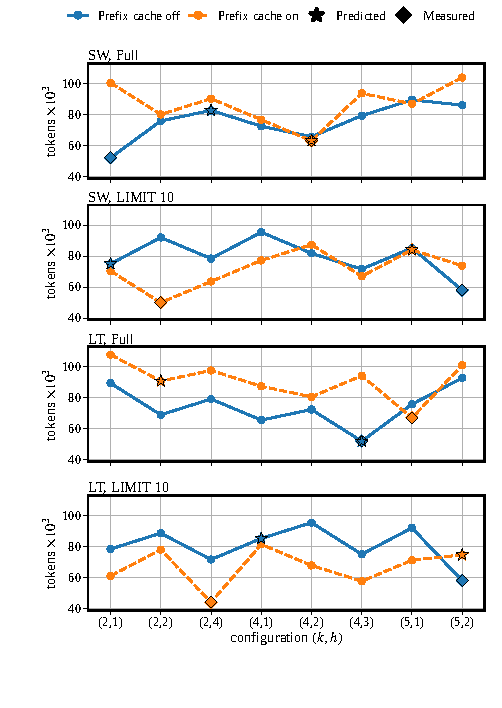
\includegraphics[width=\columnwidth]{e4a-covid-n100.pdf}
  \caption{TREC-COVID, $n{=}100$. \eFourAnote}
  \label{fig:e4a-covid-n100}
\end{figure}

\begin{figure}[t]
  \centering
  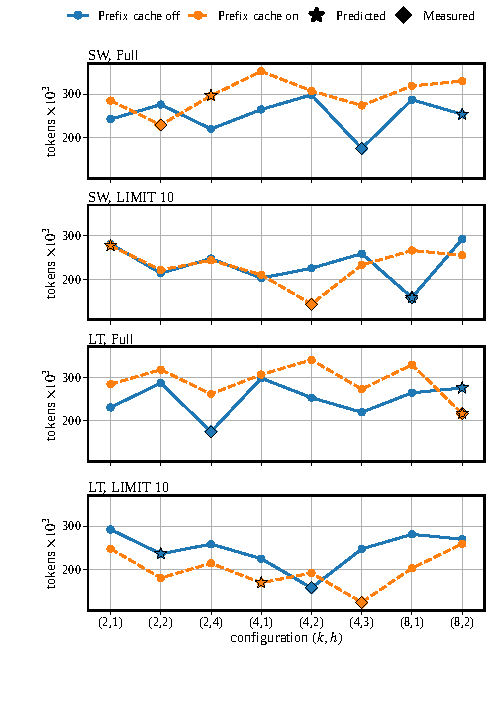
\includegraphics[width=\columnwidth]{e4a-dl20-n500.pdf}
  \caption{DL20, $n{=}500$. \eFourAnote}
  \label{fig:e4a-dl20-n500}
\end{figure}

\begin{figure}[t]
  \centering
  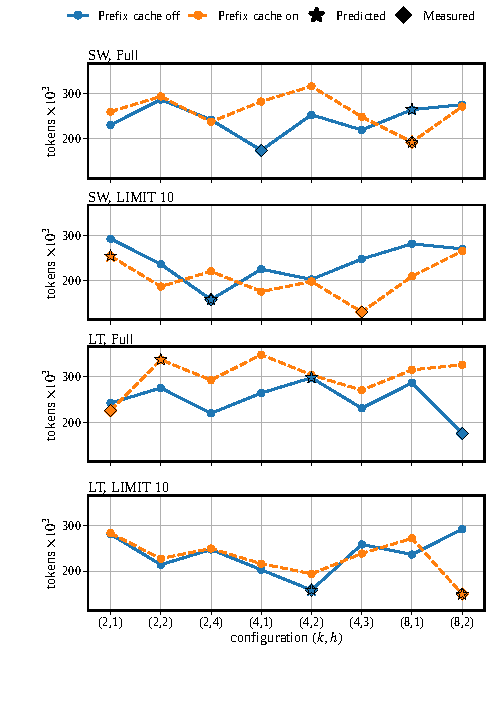
\includegraphics[width=\columnwidth]{e4a-covid-n500.pdf}
  \caption{TREC-COVID, $n{=}500$. \eFourAnote}
  \label{fig:e4a-covid-n500}
\end{figure}
}
{\graphicspath{{../experiments/figures/e4b/}}%
% E4b. Single column, no background bands, no inset.
% Not inserted into the paper. Graphic path: figures/e4b/
\begin{figure}[t]
  \centering
  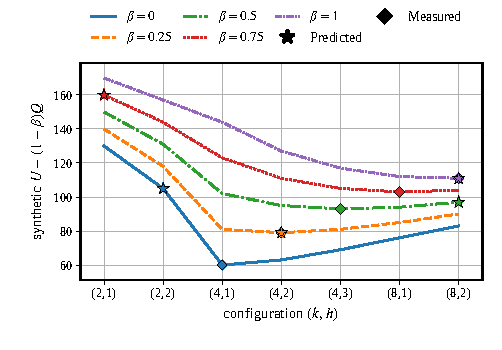
\includegraphics[width=\columnwidth]{e4b-beta.pdf}
  \caption{Synthetic On-cold slice, not a measured cost.
  Each curve is $U-(1-\beta)Q$ at the drawn $\beta$ values.
  A star is the placeholder predicted configuration and a diamond is the measured minimum of that curve; both sit on the curve.}
  \label{fig:e4b-beta}
\end{figure}
}
{\graphicspath{{../experiments/figures/e4c/}}%
% E4c. Single-column 2 by 2. Not inserted into the paper.
% Graphic path: figures/e4c/
\begin{figure}[t]
  \centering
  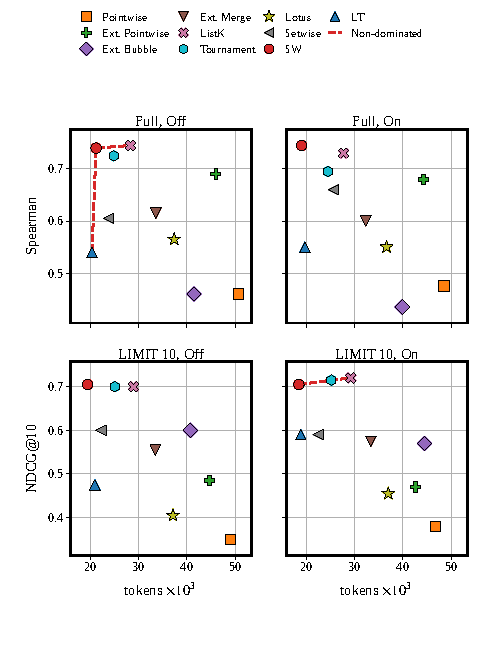
\includegraphics[width=\columnwidth]{e4c-quality-cost.pdf}
  \caption{Synthetic layout sample, not an experimental result.
  Each point is one method.
  The DL20 and COVID dataset-level placeholders are averaged with equal weight $1/2$; cost and quality are averaged separately.
  Query rows were not stored, so this is not a six-query mean and no per-query cloud is drawn.
  The two Full panels share Spearman limits, the two LIMIT~10 panels share NDCG@10 limits, and all four share the token axis.
  ListK Fig.~4 calls its red dotted curve a Pareto frontier and also runs that curve off the plotted points.
  The red dashed segments here join only non-dominated means, lower equivalent tokens and higher quality, and they stop at those means.
  They are a descriptive set, not a fit and not a significance claim.
  Full, Off joins LT, SW, and ListK.
  LIMIT~10, On joins SW, Tournament, and ListK.
  Full, On and LIMIT~10, Off each have one non-dominated mean (SW), so no segment is drawn.}
  \label{fig:e4c-quality-cost}
\end{figure}
}
\twocolumn[{%
  \graphicspath{{../experiments/figures/e5/}}%
  \begin{figure*}
    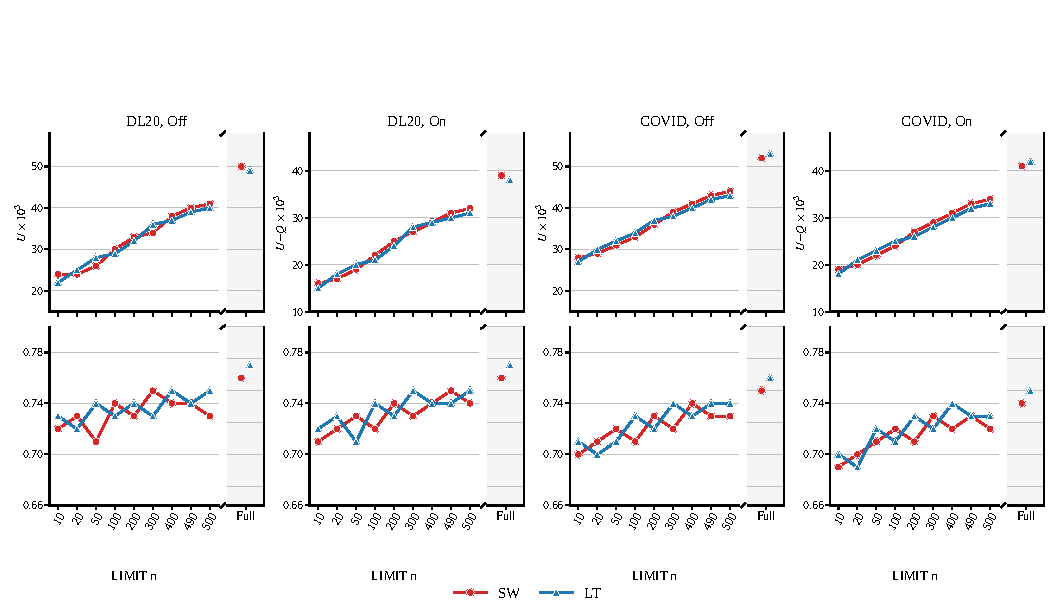
\includegraphics[width=\textwidth]{e5-limit-sweep.pdf}
    \caption{Synthetic placeholder, not a measured advantage.
    Full is a separate mode and is not joined to LIMIT~500, and it is not $K{=}510$.
    Off is equivalent input $U$; On-cold is $U{-}Q$ at $\beta{=}0$.
    The two cache states do not share a cost scale.
    Slots are equally spaced contract positions, not linear in $n$.}
    \label{fig:e5-limit-sweep}
  \end{figure*}
}]
\end{document}
